\documentclass{article}

% if you need to pass options to natbib, use, e.g.:
%     \PassOptionsToPackage{numbers, compress}{natbib}
% before loading neurips_2019

% ready for submission
 \usepackage{neurips_2019, times}
% to compile a preprint version, e.g., for submission to arXiv, add add the
% [preprint] option:
     %\usepackage[preprint]{neurips_2019}

% to compile a camera-ready version, add the [final] option, e.g.:
%   \usepackage[final]{neurips_2019}

% to avoid loading the natbib package, add option nonatbib:
%     \usepackage[nonatbib]{neurips_2019}

\usepackage[utf8]{inputenc} % allow utf-8 input
\usepackage[T1]{fontenc}    % use 8-bit T1 fonts
\usepackage{hyperref}       % hyperlinks
\usepackage{url}            % simple URL typesetting
\usepackage{booktabs}       % professional-quality tables
\usepackage{amsfonts}       % blackboard math symbols
\usepackage{nicefrac}       % compact symbols for 1/2, etc.
\usepackage{microtype}      % microtypography
\usepackage{graphicx}

\usepackage{floatrow}
\newfloatcommand{capbtabbox}{table}[][\FBwidth]
\usepackage{blindtext}
\usepackage{multirow}

\usepackage[]{algorithm2e}

\usepackage{geometry}
\usepackage{amsmath}
\usepackage{cancel}

\newcommand{\bM}{\mathbf{M}}
\newcommand{\bV}{\mathbf{V}}
\newcommand{\bv}{\mathbf{v}}
%\newcommand{\be}{\mathbf{e}}
\newcommand{\bI}{\mathbf{I}}

\title{Numerically Stable Differentiable SVD}

% The \author macro works with any number of authors. There are two commands
% used to separate the names and addresses of multiple authors: \And and \AND.
%
% Using \And between authors leaves it to LaTeX to determine where to break the
% lines. Using \AND forces a line break at that point. So, if LaTeX puts 3 of 4
% authors names on the first line, and the last on the second line, try using
% \AND instead of \And before the third author name.

\author{%
  David S.~Hippocampus\thanks{Use footnote for providing further information
    about author (webpage, alternative address)---\emph{not} for acknowledging
    funding agencies.} \\
  Department of Computer Science\\
  Cranberry-Lemon University\\
  Pittsburgh, PA 15213 \\
  \texttt{hippo@cs.cranberry-lemon.edu} \\
  % examples of more authors
  % \And
  % Coauthor \\
  % Affiliation \\
  % Address \\
  % \texttt{email} \\
  % \AND
  % Coauthor \\
  % Affiliation \\
  % Address \\
  % \texttt{email} \\
  % \And
  % Coauthor \\
  % Affiliation \\
  % Address \\
  % \texttt{email} \\
  % \And
  % Coauthor \\
  % Affiliation \\
  % Address \\
  % \texttt{email} \\
}

\begin{document}

\maketitle
% !TEX root = ../top.tex
% !TEX spellcheck = en-US

%%%%%%%%% ABSTRACT
\begin{abstract}
Singular Value Decomposition (SVD) has been widely used in deep learning, and matrix backpropagation algorithm is applied to compute the gradients. However, matrix backpropagation is numerically unstable as it involves the computation of reciprocal of the difference of arbitrary pair of eigenvalues which will cause overflow if the difference between the two eigenvalues are very small. In this paper, we propose to employ Power Iteration (PI) method to approximate the gradients of SVD during backpropagation. It can be proved that when the iteration number of PI goes to infinite, the gradients computed via PI will equal to the gradients of SVD. In other words, the gradients computed via PI can be viewed as the geometric series expansion of the gradients of SVD. The experimental results demonstrate that the proposed method, which uses SVD as forward pass and PI as backward pass, is more stable than SVD or PI. Besides, we also employs the numerically stable SVD to design a denoising layer by removing small eigenvalues during reconstruction, and it can boost the performance of the network.
\end{abstract}
% !TEX root = ../top.tex
% !TEX spellcheck = en-US

\section{Introduction}
SVD has been widely used in deep learning algorithms, such as ZCA whitening \cite{huang2018decorrelated}, second-order pooling for segmentation \cite{ionescu2015matrix}, and graph marching \cite{Zanfir_2018_CVPR}. Even though SVD is differentiable, it is very unstable for large dimension matrices. One way to alleviate the instability is to use small dimension matrix. For instance, the channels are split into smaller groups, and only the covariance matrix within each small group is computed whose dimension is 3. The other way to avoid this instability is to use power iteration to compute the eigenvectors \cite{Zanfir_2018_CVPR}. 

Power Iteration method can be employed to approximate all the eigenvalues through \textbf{deflation} procedure. In the deflation procedure, the projections of the matrix on the dominant eigenvector is removed one by one. After each removal operation, the second largest eigenvalue would become the largest one, and Power Iteration method could be used repeatedly to compute all the eigenvectors. However, power iteration method is only good at approximating the largest eigenvectors, it is a bad idea to use power iteration method to compute all the eigevectors as it brings round-off errors, and it has the premise that all eigenvalues are unique which does not strictly hold in the real application.

\subsection{Problem of SVD}
SVD has accurate and stable forward pass. However, it has accurate but \textbf{numerical unstable} gradients.
The analytic soltions of its gradients are from matrix back-propagation~\cite{ionescu2015matrix}.
	\begin{equation}
	\begin{aligned}
	\frac{\partial L}{\partial M}=V\left\{\left(\widetilde{K}^{\top} \circ\left(V^{\top} \frac{\partial L}{\partial V}\right)\right)+\left(\frac{\partial L}{\partial \Sigma}\right)_{d i a g}\right\} V^{\top}
	\end{aligned}
	\label{eq: mb}
	\end{equation}
in which $\bM$ is the covariance matrix and $V$ is the eigenvector, and $\widetilde{K}$ has the form as
\begin{equation}
	\begin{aligned}
	\widetilde{K}_{i j}=\left\{\begin{array}{ll}{\frac{1}{\lambda_{i}-\lambda_{j}},} & {i \neq j} \\ {0,} & {i=j}\end{array}\right.
	\end{aligned}
	\label{eq: mb_k}
	\end{equation}
From the equation above, we can observe that when $\lambda_{i}$ is very close to $\lambda_{j}$, the gradients will be extremely large can cause arithmetic overflow.
Let's consider an extreme case in which $\lambda_{i}-\lambda_{j}=0$, the gradients will explode as it is divided by 0. Power Iteration method could avoid this by doing Talyer expansion of the term, and the details are available in Section \ref{subsec: talyer-expansion}.

\subsection{Problem of Power Iteration}

Power Iteration (PI) method has more stable gradients than that of SVD. In fact, the gradients of PI can be viewed as a the Talyer expansion of the gradients of SVD. The details are available in Section \ref{subsec: talyer-expansion}. However, it is very numerically unstable in the forward pass, and it may fail due to a lot of reasons. 
One of the failure cases that is frequently observed during the training of Cifar10 is when the covariance matrix is singular. 

Let matrix $\bM$ be singular. In the \textbf{deflation} procedure, after removing the projections of matrix $\bM$ on the eigenvectors with non-zero eigenvalues, we obtain $\widetilde{\bM}$, which is a close-to-zero matrix with round-off errors. In such situation, the eigenvector $\widetilde{V}$ could be arbitrary and the corresponding eigenvalue computed by the Rayleigh quotient $\frac{\widetilde{V}^{\top} \widetilde{\bM} \widetilde{V}}{\widetilde{V}^{\top}  \widetilde{V}}$ will be incorrect. Such case is catastrophic during the model training process as it will cause arithmetic overflow and destroy the model parameters during backpropagation. One real failure case caught during the training of Cifar10 is shown in the supplementary material.

Another unstable factor of PI is when the eigenvalues are not unique. If two eigenvalues are very close to each other, it requires an extremely large number of iterations to approximate the correct eigenvectors, and this is prohibitive in the real applications. The limited number of iterations can hardly compute the correct eigenvectors and will lead to instability in the training. One real case study is shown in the experiments. The relationship between the number of power iteration and the approximated eigenvectors is also illustrated in Section ***. SVD is free of these problems.

To sum up, SVD has the problem during the backpropagation while PI has the problem of computing eigenvectors in the forward pass.
To solve the problems of both SVD and PI, we propose to combine these two methods together, that is, SVD is used to compute the forward pass and PI is used to compute the gradients in the backward pass.
\section{Options to Compute SVD.}

\begin{itemize}
\item Given input covariance matrix $\bM$, use \textbf{Eigen Decomposition} or \textbf{Singular Value Decomposition (SVD)} Operation as forward computation, and use the analytic solution of its gradient for backward propogation.
\item Given input covariance matrix $\bM$, vectors with random values $[\bv_1^{1}, \bv_2^{1}, ...]$, use \textbf{Power Iteration} as forward computation, and use its gradient for backward propogation.
\item Given input covariance matrix $\bM$, vectors with random values $[\bv_1^{1}, \bv_2^{1}, ...]$, use \textbf{Eigen Decomposition} or \textbf{SVD} Operation as forward computation, and use \textbf{Power Iteration} to approximate the analytic solutions of the gradient for backward propogation.
\end{itemize}

Usually, people choose either option 1 or option 2 to compute SVD, but both of them have problems.
In option 1, \textbf{Eigen Decomposition} or \textbf{Singular Value Decomposition (SVD)}, the analytic solutions of the gradient sometimes causes NaN problem when there are two or more eigenvalues are too close to each other.
In option 2, if the two eigenvalues are very close, eigenvectors could not be computed precisely with limited power iteration number. Thus, during backprorogation, the derivatives will be very inaccurate and destroy the parameters of model, and cause numerical instability in the training process.

In this paper, we propose to using option 3. During forward pass, we use \textbf{SVD} to compute the eigenvalues. 
SVD is numerically more stable than eigendecomposition \cite{nakatsukasa2013stable} as SVD implementation employs a divide-and-conquer strategy, while the eigendecomposition uses QR algorithm. 
During backpropogation, we employ \textbf{Power Iteration} method to compute the numerical solutions of the covariance matrix $\bM$ gradient.
In \textbf{sections} \ref{sec: pi} \& \ref{sec: mbp}, we will prove that when the iteration number goes to infinite, the accumulated gradients (\emph{i.e.} numerical solution) from the \textbf{Power Iteration} method is exactly the same with the analytic solution of the gradient.

\section{Approximate SVD gradient with Power Iteration in backpropogation}
In the following 2 subsections, we will prove that when the gradient computed from Power Iteration equals to the gradients computed from SVD.
	\subsection{Gradient of Power Iteration}
	\label{sec: pi}
	To compute the leading eigenvector $\bv$ of $\bM$, Power Iteration uses the following standard formula,
	\begin{equation}
	\bv^{(k)} = \frac{\bM\bv^{(k-1)}}{\| \bM\bv^{(k-1)} \|},
	\end{equation}
	in which $\| {\cdot} \|$ denotes the $l_2$ norm, and $v^{(0)}$ is usually initialized randomly with  $\|v^{(0)}\|{=}1$.
    Its gradient is as follows~\cite{ye2017dynamic},
	\begin{equation}
	\begin{aligned} 
	\frac{\partial L}{\partial \bM} &=\sum_{k} \frac{\left(\bI-\bv^{(k+1)} \bv^{(k+1)\top}\right)}{\left\|\bM \bv^{(k)}\right\|} \frac{\partial L}{\partial \bv^{(k+1)}} \bv^{(k)\top} \\
	\frac{\partial L}{\partial \bv^{(k)}} &=\bM \frac{\left(\bI-\bv^{(k+1)} \bv^{(k+1)\top}\right)}{\left\|\bM \bv^{(k)}\right\|} \frac{\partial L}{\partial \bv^{(k+1)}} 
	\end{aligned}
	\end{equation}

In the forward pass, we use SVD to compute the eigenvector, $\bv$.
If we feed $\bv$ directly to the power iteration method as initial value, we will have $\bv {=} \bv^{(0)} {\approx}\bv^{(1)} {\approx} \bv^{(2)}{\approx} \cdots {\approx}\bv^{(k)} \cdots {\approx}\bv^{(K)}$.
After introducing $\frac{\partial L}{\partial \bv^{(k)}}, \; k=1,2, \cdots, K$ into $\frac{\partial L}{\partial \bM}$, we can obtain
	\begin{equation}
	\frac{\partial L}{\partial \bM}
	 = \left( \frac{\left(\bI-\bv \bv^{\top}\right)}{\left\|\bM \bv\right\|}  +
	 \frac{\bM \left(\bI-\bv \bv^{\top}\right)}{\left\|\bM \bv\right\|^{2}}  + \cdots +
	 \frac{\bM^{K-1} \left(\bI-\bv \bv^{\top}\right)}{\left\|\bM \bv\right\|^{K}} \right) \frac{\partial L}{\partial \bv^{(K)}}
	\bv^{\top}
	\label{eq: pi_pytorch}
	\end{equation}	

The deduction details of Eq.\ref{eq: pi_pytorch} is available in the supplementary material.
Eq.\ref{eq: pi_pytorch} is the form we adopt to compute the gradients of SVD, and we set $K{=}19$.


\subsection{Relationship between Gradients of Power Iteration and SVD}
In this subsection, we are going to prove that the gradients of SVD and Power Iteration are equivalent. In the end of this section, we can observe that when the number of the iterations goes to infinity, the gradients of Power Iteration can be written as the same form as the one of SVD.
\subsubsection{Gradients of Power Iteration}
The gradients of Power Iteration could be formulated into another form using the following properties.
	\begin{equation}
	\begin{aligned}
	\bM & = \bV \Sigma \bV^{\top} & = & \lambda_{1}\bv_{1}\bv_{1}^{\top} + \lambda_{2}\bv_{2}\bv_{2}^{\top} + \cdots +  \lambda_{n}\bv_{n}\bv_{n}^{\top}, \\
	\bM^{k} & = \bV \Sigma^{k} \bV^{\top} & = & \lambda_{1}^{k}\bv_{1}\bv_{1}^{\top} +  \lambda_{2}^{k}\bv_{2}\bv_{2}^{\top} + \cdots + \lambda_{n}^{k}\bv_{n}\bv_{n}^{\top},\\
	\end{aligned}
	\label{eq: term_k}
	\end{equation}
	and $\left\|\bM\bv\right\| = \left\| \lambda \bv \right\|= \lambda$,
	in which $\bv = \bv_1$ is the leading eigenvector and $\lambda=\lambda_1$ is the leading eigenvalue.
	By introducing Eq.\ref{eq: term_k} into Eq.\ref{eq: final-form}, the derivative can be further formulated as
	
	\begin{equation}
	\begin{aligned} 
	\frac{\partial L}{\partial \bM}
	& =\left( \frac{\left(\bI-\bv_1 \bv_1^{\top}\right)}{\left\|\bM \bv_1\right\|}  +
	 \frac{\bM \left(\bI-\bv_1 \bv_1^{\top}\right)}{\left\|\bM \bv_1\right\|^{2}}  + \cdots +
	 \frac{\bM^{K-1} \left(\bI-\bv_1 \bv_1^{\top}\right)}{\left\|\bM \bv_1\right\|^{K}} \right)
	 \frac{\partial L}{\partial \bv_1^{(K)}}\bv_1^{\top} \\
	&=\left( \frac{\left(\bI-\bv_1 \bv_1^{\top}\right)}{\left\|\bM \bv_1\right\|} +
	\frac{\left(\bM-\lambda \bv_1 \bv_1^{\top}\right)}{\left\|\bM \bv_1\right\|^2}  + \cdots +
	\frac{\left(\bM^{K-1} - \lambda^{K-1}\bv_1\bv_1^{\top}\right)}{\left\|\bM \bv\right\|^{K}} \right) \frac{\partial L}{\partial \bv_1^{(K)}} \bv_1^{\top}\\
	&=\left( \frac{\left(\sum_{i=2}^{n}\bv_{i}\bv_{i}^{\top}\right)}{\lambda_1}      +
	\frac{\left(\sum_{i=2}^{n}\lambda_{i}\bv_{i}\bv_{i}^{\top}\right)}{ \lambda_{1}^{2}} +  \cdots +
	\frac{\left(\sum_{i=2}^{n}\lambda_{i}^{K-1}\bv_{i}\bv_{i}^{\top}\right)}{\lambda_{1}^{K}} \right) \frac{\partial L}{\partial \bv_1^{(K)}}
	\bv^{\top}\\
	&=\left(\sum_{i=2}^{n}\left(
	\frac{1}{\lambda_{1}} +
	\frac{1}{\lambda_{1}}\left(\frac{\lambda_{i}}{\lambda_{1}}\right)^{1} +
	\frac{1}{\lambda_{1}}\left(\frac{\lambda_{i}}{\lambda_{1}}\right)^{2} + \cdots +
	\frac{1}{\lambda_{1}}\left(\frac{\lambda_{i}}{\lambda_{1}}\right)^{K-1}
	\right)\bv_{i}\bv_{i}^{\top}
	\right)\frac{\partial L}{\partial \bv_{1}^{(K)}}\bv_{1}^{\top}\\
	\end{aligned}
	\label{eq: geo-prog-series}
	\end{equation}
	In Eq.\ref{eq: geo-prog-series}, we have a geometric progression series.
	Given that $${1 - (\frac{\lambda_{i}}{\lambda_{1}})^k \rightarrow 1}, \text{when} \; k\rightarrow\infty, \vert \frac{\lambda_{i}}{\lambda_{1}} \vert<1,$$
	then we have
	\begin{equation}
	\frac{1}{\lambda_{1}} +
	\frac{1}{\lambda_{1}}\left(\frac{\lambda_{i}}{\lambda_{1}}\right)^{1} +
	\frac{1}{\lambda_{1}}\left(\frac{\lambda_{i}}{\lambda_{1}}\right)^{2} + \cdots +
	\frac{1}{\lambda_{1}}\left(\frac{\lambda_{i}}{\lambda_{1}}\right)^{k-1} = \frac{\frac{1}{\lambda_{1}}(1- (\frac{\lambda_{i}}{\lambda_{1}})^k)} {1 - \frac{\lambda_{i}}{\lambda_{1}}} 
	\rightarrow  \frac{\frac{1}{\lambda_{1}}}
	{1 - \frac{\lambda_{i}}{\lambda_{1}}}, \text{when} \; k\rightarrow\infty.
	\label{eq: geo-prog-series-deduction}
	\end{equation}
	
	Introducing Eq.\ref{eq: geo-prog-series-deduction} to Eq.\ref{eq: geo-prog-series}, we can obtain	
	\begin{equation}
	\frac{\partial L}{\partial \bM}
	=\left(\sum_{i=2}^{n}\left(
	\frac{\frac{1}{\lambda_{1}}}
	{1 - \frac{\lambda_{i}}{\lambda_{1}}}
	\right)
	\bv_{i}\bv_{i}^{\top}
	\right)\frac{\partial L}{\partial \bv_{1}^{(k)}}\bv_{1}^{\top}
	=\left(\sum_{i=2}^{n}
	\frac{\bv_{i}\bv_{i}^{\top}}
	{\lambda_{1} - \lambda_{i}}
	\right)\frac{\partial L}{\partial \bv_{1}^{(k)}}\bv_{1}^{\top}
	\label{eq: final-form}
	\end{equation}
	
	\subsubsection{Matrix Back-propagation}
	\label{sec: mbp}
	Eq.\ref{eq: mb} shows the analytic soltions of the gradients of matrix back-propagation~\cite{ionescu2015matrix}.
	It could be further formulated as the following form:
	\begin{equation}
	\frac{\partial L}{\partial M}
	=\sum_{i=2}^{n}\frac{1}{\lambda_{1}-\lambda_{i}}\bv_{i}\bv_{i}^{\top}\frac{\partial L}{\partial \bv_{1}}\bv_{1}^{\top}
	+ \cancel{\frac{\partial L}{\partial \lambda_i}\bv_i\bv_i^{\top}}
	\label{eq: mb-pi-form}
	\end{equation}
   We avoid using eigenvalues in the forward pass by formulating it as a function of eigenvectors using the Rayleigh quotient $\frac{\bv^{\top} \bM \bv}{\bv^{\top}  \bv}$, such that it has no gradients, which means $\frac{\partial L}{\partial \Sigma}$ could be ignored. The deduction details of Eq.\ref{eq: mb-pi-form} is available in the supplementary material.

Now we have shown that the partial derivative of \emph{e.g.}, $\bv_1$ computed from Power Iteration and SVD share the same form when $k\rightarrow \inf$.
Similar deductions could be done for  $\bv_i, i=2,3,...$.
This justifies that we could use power iteration method during backpropogation to approximate the gradients of SVD, but we need to choose an approximate iteration number.

\subsection{Impact of the Number of Power Iterations}
\label{subsec: talyer-expansion}
The power iteration number $K$ has a fundamental influence to the approximated gradients. In fact, it controls the upper bond of the gradients.

Eq.\ref{eq: geo-prog-series} can be viewed as the geometric series expansion of Eq.\ref{eq: mb-pi-form}.
When the covarriance matrix is singular with two same eigenvalues $\lambda_1 = \lambda_i$, the gradients computed from Eq.\ref{eq: mb-pi-form} will go to $\pm \infty$ as the denominator is 0. However, Eq.\ref{eq: geo-prog-series} naturally brings an upper bond to avoid this problem as shown in the following deduction,

	\begin{equation}
	\begin{aligned}
	\frac{\partial L}{\partial M} & = \sum_{i=2}^{n}\frac{1}{\lambda_{1}-\lambda_{i}}\bv_{i}\bv_{i}^{\top}\frac{\partial L}{\partial \bv_{1}}\bv_{1}^{\top} \\
	&\approx \left(\sum_{i=2}^{n}\left(
	\frac{1}{\lambda_{1}} {+}
	\frac{1}{\lambda_{1}}\left(\frac{\lambda_{i}}{\lambda_{1}}\right)^{1} {+}
	\frac{1}{\lambda_{1}}\left(\frac{\lambda_{i}}{\lambda_{1}}\right)^{2} {+} \cdots {+}
	\frac{1}{\lambda_{1}}\left(\frac{\lambda_{i}}{\lambda_{1}}\right)^{K-1}
	\right)\bv_{i}\bv_{i}^{\top}
	\right)\frac{\partial L}{\partial \bv_{1}}\bv_{1}^{\top}
	\end{aligned}
	\end{equation}
	
	\begin{equation}
	\begin{aligned}
	\left\| \frac{\partial L}{\partial M} \right\|
	& \leq \left\| \sum_{i=2}^{n}\left(
	\frac{1}{\lambda_{1}} {+}
	\frac{1}{\lambda_{1}}\left(\frac{\lambda_{i}}{\lambda_{1}}\right)^{1} {+}
	\frac{1}{\lambda_{1}}\left(\frac{\lambda_{i}}{\lambda_{1}}\right)^{2} {+} \cdots {+}
	\frac{1}{\lambda_{1}}\left(\frac{\lambda_{i}}{\lambda_{1}}\right)^{K-1}
	\right)\bv_{i}\bv_{i}^{\top}
	\right\| \left\|  \frac{\partial L}{\partial \bv_{1}} \right\|  \left\|  \bv_{1}^{\top} \right\| \\
	& \leq \left\| \sum_{i=2}^{n}\left(
	\frac{1}{\lambda_{1}} {+}
	\frac{1}{\lambda_{1}} {+}
	\frac{1}{\lambda_{1}} {+} \cdots {+}
	\frac{1}{\lambda_{1}}
	\right)\bv_{i}\bv_{i}^{\top}
	\right\| \left\|  \frac{\partial L}{\partial \bv_{1}} \right\|  \left\|  \bv_{1}^{\top} \right\| \\
	 & \leq \sum_{i=2}^{n} \left\| 
	\frac{K}{\lambda_{1}}
	\bv_{i}\bv_{i}^{\top}
	\right\| \left\|  \frac{\partial L}{\partial \bv_{1}} \right\|  \left\|  \bv_{1}^{\top} \right\|  
	\leq \frac{nK}{\lambda_{1}} \left\|  \frac{\partial L}{\partial \bv_{1}} \right\|
	\end{aligned}
	\end{equation}

Till now, we have obtain the upper bound of $\left\| \frac{\partial L}{\partial M} \right\|$. However, if $\lambda_{1} = 0$, the upper bound will also become $\infty$. To avoid this, we do the following operation to the covariance matrix $\bM = \bM + \epsilon I$, in which $I$ is an identity matrix. As $\bM$ is a covariance matrix which is positive semi-definite, the eigenvalues of $\bM + \epsilon I$ can be guaranteed to be larger than $\epsilon$.
Thus, the upper bound can be written as 

\begin{equation}
	\begin{aligned}
	\left\| \frac{\partial L}{\partial (M+\epsilon I) } \right\|
	\leq \frac{nK}{\epsilon} \left\|  \frac{\partial L}{\partial \bv_{1}} \right\|
	\end{aligned}
\end{equation}
in which $n$ is the dimension of the matrix and $K$ is the power iteration number. In the following experiments, we set $\epsilon = 10^{-4}$, and $K=19$.
In the following, we will explain why $K$ is set to 19.

\subsection{Select Appropriate Power Iteration Number K}

\begin{figure}[!htb]
\begin{center}
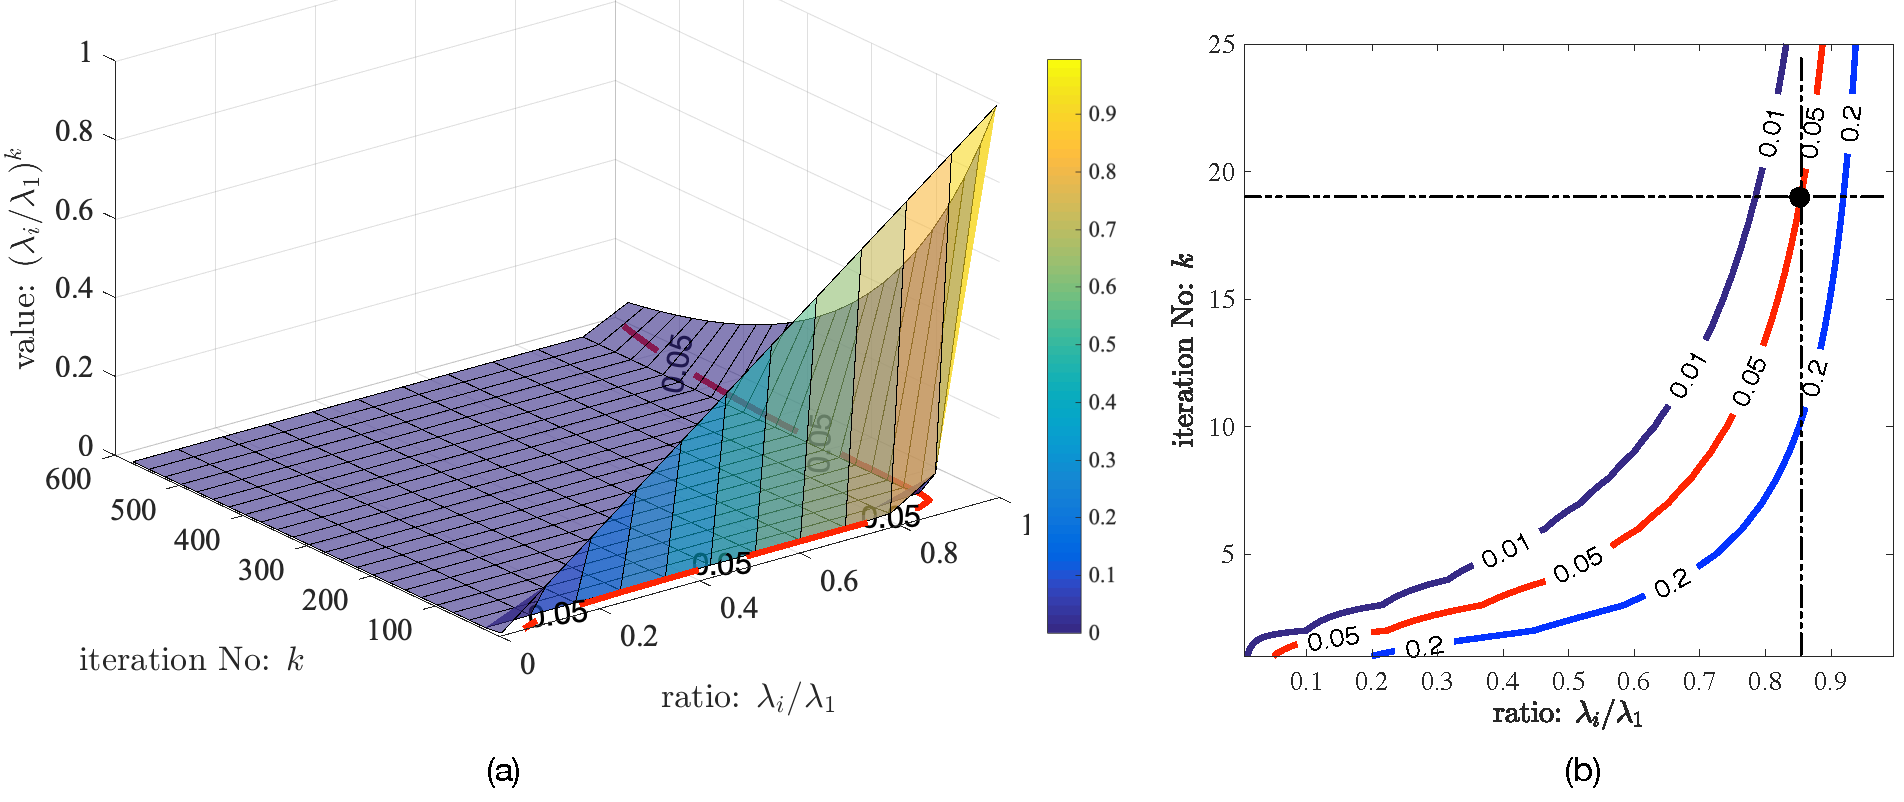
\includegraphics[width=\linewidth]{ratio-k.pdf}
\end{center}
\caption{(a) shows how the value of $(\lambda_k/\lambda_1)^k$ changes \emph{w.r.t.} the eigenvalue ratio $\lambda_k/\lambda_1$ and iteration number $k$. (b) shows the contour of curved surface in (a).}
\label{fig: curve}
\end{figure}

Fig. \ref{fig: curve} shows how the value of $(\lambda_i/\lambda_1)^k$ evolves with different power iteration number $k$ and ratio~$\lambda_i/\lambda_1$. We need to select appropriate $k$ for different $\lambda_i/\lambda_1$ given $(0 < \lambda_i/\lambda_1 \leq 1)$. 

Let's assume $(\lambda_i/\lambda_1)^k<0.05$ being a good approximation to $(\lambda_i/\lambda_1)^k=0$. Then we have
\begin{equation}
(\lambda_i/\lambda_1)^k<0.05 \Leftrightarrow k\; \text{ln}(\lambda_i/\lambda_1) < \text{ln}(0.05) \Leftrightarrow k \geq \frac{\text{ln}(0.05)}{\text{ln}(\lambda_i/\lambda_1)}.
\end{equation}
The minimum value of $k$ to satisfy $(\lambda_i/\lambda_1)^k<0.05$ is $k = \lceil \frac{\text{ln}(0.05)}{\text{ln}(\lambda_i/\lambda_1)} \rceil$.

\begin{table}[!htb]
\begin{centering}
\setlength\tabcolsep{4pt}
\begin{tabular}{ccccccccccccccc}
\hline
$\lambda_i/\lambda_1$ & 0.1& 0.2& 0.3 & 0.4 & 0.5 & 0.6 & 0.7 & 0.8 & \textbf{0.85} & 0.9 & 0.95 & 0.99 & 0.995 & 0.999 \\ \hline
$k = \lceil \frac{\text{ln}(0.01)}{\text{ln}(\lambda_i/\lambda_1)} \rceil $   & 2 & 2 & 3 & 4 & 5 & 6 & 9 & 14  & \textbf{19}   & 29  & 59   & 299  & 598   & 2995  \\ \hline
\end{tabular}
\caption{The minimum value of $k$ we need to guarantee $(\lambda_i/\lambda_1)^k<0.05$.}
\label{tab: kmin}
\end{centering}
\end{table}

Table \ref{tab: kmin} shows the minimum number of iterations we need to guarantee that the assumption holds. We can observe that when the two eigenvalues are very close to each other \emph{e.g.}, $\lambda_i/\lambda_1=0.999$, we need about 3000 iterations to achieve a good approximation. However, in practice, the case is very rare, and we set power iteration number to be 19. This will satisfy most of the cases. Besides, two very close eigenvalues usually leads to overflow according to Eq.\ref{eq: final-form} as the denominator $\lambda_1 - \lambda_i$ would be close to 0, but with our approximation, this problem could be avoided, and our method is more numerical stable.

\subsection{Practical Issues}
There are several practical issues when use Power Iteration to approximate the gradients of SVD.
In practice, take ZCA whitening for example, we use the following steps to compute the forward pass.

\begin{algorithm}[H]
 \KwData{$\mu=Avg(X)$, $\widetilde{X}=X-\mu$, $\bM=\widetilde{X}\widetilde{X}^{\top}+\epsilon I$, ($X \in R^{c\times nhw}$);}
 \KwResult{$V^{\top}\Lambda V=SVD(\bM)$; $\Lambda = diag(\lambda_1, \lambda_2, ..., \lambda_n)$; $V=\left[\bv_1,\bv_2,\cdots, \bv_n\right]$; $\gamma_i=\frac{\sum_{k=1}^i\lambda_k}{\sum_{k=1}^n\lambda_k}$; }
 initialization:$running_{\mu}=0$, $running_{S}=I$, $\widetilde{\bM} = \bM$,  $rank=1$\; 
 \For{$i=1:n$}{
  $\bv_i$ = Power Iteration($\widetilde{\bM}, \bv_i$);
  $\widetilde{\lambda_i} = \frac{\bv_i^{\top}\widetilde{\bM}\bv_i}{\bv_i^{\top}\bv_i}$;
  $\widetilde{\bM} = \widetilde{\bM} -  \widetilde{\bM}\bv_i\bv_i^{\top}$\;
  \eIf{$\lambda_i \leq \epsilon$  or  $\frac{\left| \widetilde{\lambda_i}-\lambda_i \right|}{\lambda_i} \geq 0.1$  or  $\gamma_i \geq (1-0.0001)$}{
   break\;
   }{$rank = i$, $\widetilde{\Lambda} = [\widetilde{\lambda_1}, \cdots, \widetilde{\lambda_i}]$.}
   }
   {truncate eigenvector matrix: $\widetilde{V}=[\bv_1, \bv_2, \cdots, \bv_{rank}]$
   compute subspace: $S=\widetilde{V}(\widetilde{\Lambda})^{-\frac{1}{2}}\widetilde{V}^{\top}$\;
   compute ZCA output: $X=S\widetilde{X}$\;
   update $running_{S} = momentum \cdot S + (1-momentum) \cdot running_{S}$\;
   update $running_{\mu} = momentum \cdot \mu + (1-momentum) \cdot running_{\mu}$\;
   }

 \caption{Forward Pass of ZCA whitening in Practice.}
 \label{alg: svd-foward}
\end{algorithm}


The first issue is that in the forward pass, the eigenvalues computed using SVD may be inaccurate.
Remember that to increase the stability, a small value $\epsilon$ is added to the diagonal axis of the covarraince matrix.
In this way, all the eigenvalues should be greater or equal to $\epsilon$. However, this is not the case when we use float precision instead of double precision.
To solve this problem, we employ truncated SVD.
When we found that the computed eigenvalue $\lambda_i \leq \epsilon$, we will truncate this $\lambda_i$ and its following $\lambda_{i+1}, \cdots,\lambda_{n}$.

The second issues is the approximation of the eigenvalues computed using $\widetilde{\lambda_i} = \frac{\bv^{\top} \widetilde{\bM} \bv}{\bv^{\top}\bv}$.
Because of the round-off error from $\widetilde{\bM} = \widetilde{\bM} -  \widetilde{\bM}\bv_i\bv_i^{\top}$, $\widetilde{\lambda_i}$ may be inaccurate and sometimes may be negative.
To avoid using incorrect eigenvalues, we also need to truncate it.

These two practical issues are the breaking conditions $\lambda_i \leq \epsilon$, $\frac{\widetilde{\lambda_i}-\lambda_i}{\lambda_i} \geq 0.1$ defined in Alg.\ref{alg: svd-foward}. Besides, we have added another constraint $\gamma_i \geq (1-0.0001)$ which means if the remaining energy preserved in $\widetilde{\bM}$ is less than 0.0001, we will also do the truncation as the remaining information is too trivial.
\section{Experiments}
We apply SVD into two tasks, one of which is ZCA whitening and the other one is PCA denoising.
\subsection{ZCA Whitening}

The algorithm of ZCA whitening follows the big framework defined in Alg.\ref{alg: svd-foward}.
Following \cite{huang2018decorrelated}, the affine transformation operation is also kept. For simplicity, we did not show it in Alg.\ref{alg: svd-foward}.
For ZCA whitening, we have tested our algorithm on both CIFAR10 and CIFAR100 datasets.

\begin{table}[!htb]
\begin{tabular}{|l|c|c|c|c|c|c|}
\hline
Methods                 & Error & ZCA-G1                 & ZCA-G2        & ZCA-G4        & ZCA-G8        & ZCA-G16       \\ \hline
\multirow{2}{*}{SVD}    & Min   & NaN                    & NaN           & NaN           & NaN           & 4.43             \\ \cline{2-7} 
                        & Mean  & NaN                    & NaN           & NaN           & NaN           & 4.53$\pm$0.15         \\ \hline
\multirow{2}{*}{PI}     & Min   & -                      & -             & -             & -             & -             \\ \cline{2-7} 
                        & Mean  & -                      & -             & -             & -             & -             \\ \hline
\multirow{2}{*}{SVD-PI} & Min   & 4.44                   & 4.46          & \textbf{4.40} & 4.43          & 4.59          \\ \cline{2-7} 
                        & Mean  & \textbf{4.59$\pm$0.09} & 4.64$\pm$0.15 & 4.63$\pm$0.14 & 4.62$\pm$0.18 & 4.71$\pm$0.11 \\ \hline
\end{tabular}
\end{table}


\begin{table}[!htb]
\begin{centering}
\setlength\tabcolsep{2.5pt}
\begin{tabular}{|l|l|c|c|c|c|c|c|}
\hline
\multicolumn{1}{|c|}{Methods}                                                & Error & BN             & G1                  & G2                  & G4         & G8         & G16        \\ \hline
\multirow{2}{*}{\begin{tabular}[c]{@{}l@{}}CIFAR100\\ ResNet18\end{tabular}} & Min   & 21.68          & 21.04                   & 21.36                   & 21.14          & 21.15          & \textbf{21.03} \\ \cline{2-8} 
                                                                             & Mean  & 21.85$\pm$0.14 & \textbf{21.39$\pm$0.23} & 21.58$\pm$0.27          & 21.45$\pm$0.25 & 21.56$\pm$0.35 & 21.51$\pm$0.28 \\ \hline
\multirow{2}{*}{\begin{tabular}[c]{@{}l@{}}CIFAR100\\ ResNet50\end{tabular}} & Min   & 20.79          & 19.28                   & \textbf{19.24}          & 19.78          & 20.15          & 20.66          \\ \cline{2-8} 
                                                                             & Mean  & 21.62$\pm$0.65 & 19.94$\pm$0.44          & \textbf{19.54$\pm$0.23} & 19.92$\pm$0.12 & 20.59$\pm$0.58 & 20.98$\pm$0.31 \\ \hline
\end{tabular}
\end{centering}
\caption{CIFAR100 results with ResNet18 and ResNet50 as the backbone.}
\label{tab: cifar100}
\end{table}



\subsection{PCA denoising}

In the experiment, within the PCA denoising layer, we remove the noise in the feature maps by only selecting its top-$k$ eigenvectors to reconstruct the input feature maps.
We first reshape the input feature maps $X_{n {\times} c {\times} h {\times} w}$ to $X_{c {\times} nhw}$, and compute the covariance matrix $Var(X) =\frac{XX^{\top}}{nhw-1}$.
The constraint for $k$ is that $\frac{\sum_{i=1}^k\lambda_i}{\sum_{i=1}^n\lambda_i} \geq 0.95$, which means that $95\%$ of the information is preserved and the rest of the information which is lower than $5\%$ is removed. 
In practice, $k$ is relatively small compared with channel number $c$. For instance, on Cifar10 dataset, after the first convolutional layer in ResNet18 which has the channel 64, we observe that \\
more than $95\%$ of the information could be preserved when $k=7$; \\
more than $99\%$ of the information could be preserved when $k=15$; \\
more than $99.5\%$ of the information could be preserved when $k=31$. 

\subsubsection{Percentage of Preserved Information VS Performance}

\begin{figure}[!htb]
\begin{floatrow}
\ffigbox[1.1\FBwidth]{%
  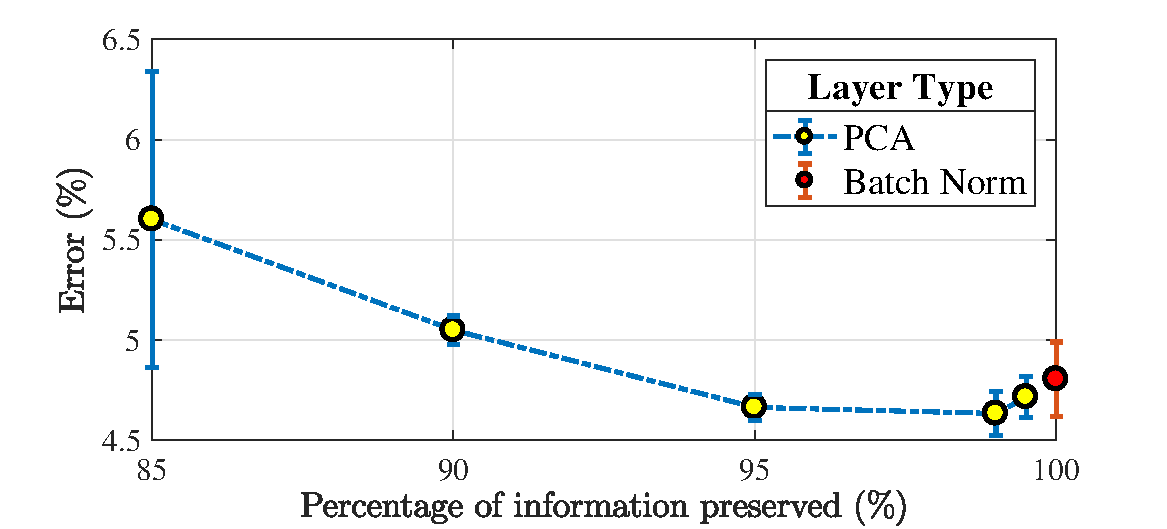
\includegraphics[width=\linewidth]{information.pdf}
}
{%
  \caption{Preserved information VS Performance.}%
}
\capbtabbox[.9\Xhsize]{%
\begin{tabular}{cc}
\hline
Percentage (\%) & Error (\%) \\ \hline
85              & $5.60\pm0.74$  \\ \hline
90              & $5.05\pm0.07$  \\ \hline
95              & $4.67\pm0.06$  \\ \hline
99              & $\mathbf{4.63\pm0.11}$  \\ \hline
99.5            & $4.72\pm0.10$  \\ \hline
100             & $4.81\pm0.19$  \\ \hline
\\
\end{tabular}
}{%
  \caption{Performance Comparison}%
}
\end{floatrow}
\end{figure}

\subsubsection{Number of EigenVectors VS Performance}

\begin{figure}[!htb]
\begin{floatrow}
\ffigbox[1.1\FBwidth]{%
  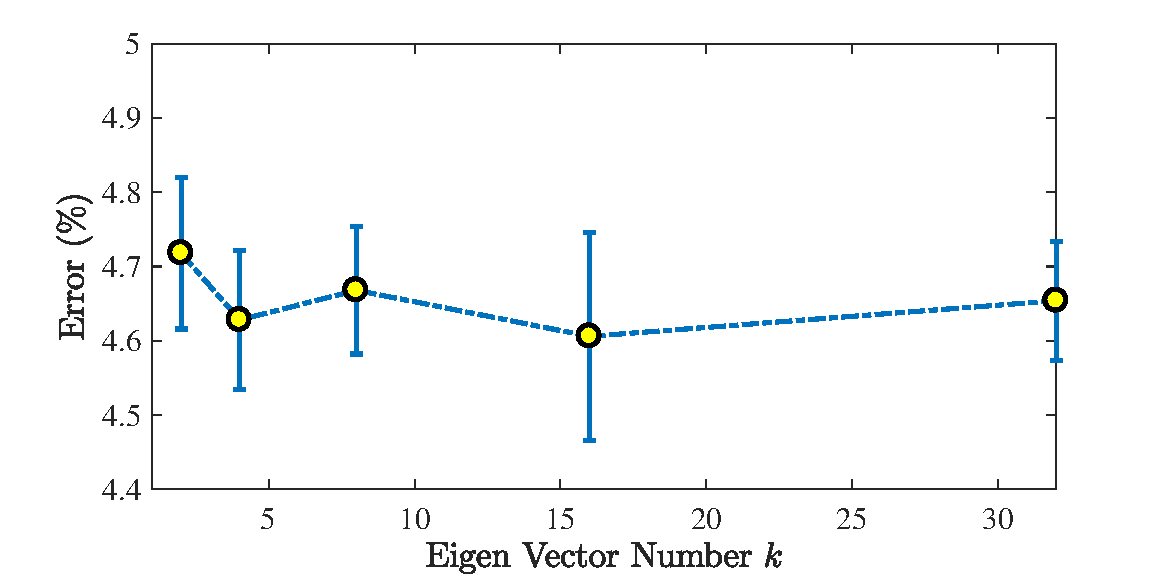
\includegraphics[width=\linewidth]{eig.pdf}
}
{%
  \caption{Eigen-vector No. VS Performance.}%
}
\capbtabbox[.9\Xhsize]{%
\begin{tabular}{cc}
\hline
Eig-vector No. & Error (\%) \\ \hline
2              & $4.72 \pm 0.10$  \\ \hline
4              & $4.63 \pm 0.09$  \\ \hline
8              & $4.67 \pm 0.09$ \\ \hline
16            & $4.61 \pm 0.14$  \\ \hline
32             & $4.65 \pm 0.08$  \\ \hline
\\
\end{tabular}
}{%
  \caption{Performance Comparison}%
}
\end{floatrow}
\end{figure}

\subsubsection{Number of Power Iterations VS Performance}

\begin{figure}[!htb]
\begin{floatrow}
\ffigbox[1.1\FBwidth]{%
  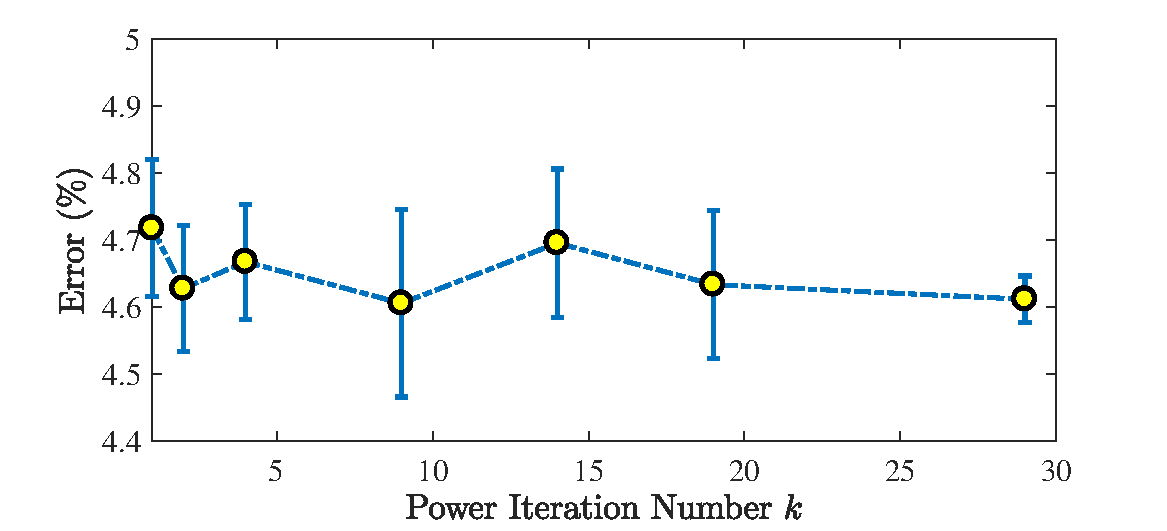
\includegraphics[width=\linewidth]{pi.pdf}
}
{%
  \caption{Power Iteration No. VS Performance.}%
}
\capbtabbox[.9\Xhsize]{%
\begin{tabular}{cc}
\hline
Power Iteration No. & Error (\%) \\ \hline
1              & $4.72 \pm 0.10$  \\ \hline
2              & $4.63 \pm 0.09$  \\ \hline
4              & $4.67 \pm 0.09$  \\ \hline
9              & $4.61 \pm 0.14$ \\ \hline
14            & $4.69 \pm 0.11$  \\ \hline
19             & $4.63 \pm 0.11$  \\ \hline
29             & $\mathbf{4.61 \pm 0.03}$  \\ \hline
\end{tabular}
}{%
  \caption{Performance Comparison}%
}
\end{floatrow}
\end{figure}

%\begin{table}[!htb]
%\begin{centering}
%\begin{tabular}{|l|c|c|c|c|}
%\hline
%Norm Methods          & BN        & PCA(PI)  & PCA(SVD) & PCA(SVD+PI) \\ \hline
%Minimum Error         & 4.66       & 5.05   & NaN   &\textbf{4.58}\\ \hline
%Mean Error (4) & $4.81{\pm}0.19$ &$5.35{\pm}0.25$ & NaN &$\mathbf{4.67{\pm}0.06}$ \\ \hline
%\end{tabular}
%\caption{CIFAR-10 test errors using ResNet18 (single PCA/ZCA normalization layer).}
%\end{centering}
%\end{table}

\begin{figure}[!htb]
\begin{floatrow}
\ffigbox[0.9\FBwidth]{%
  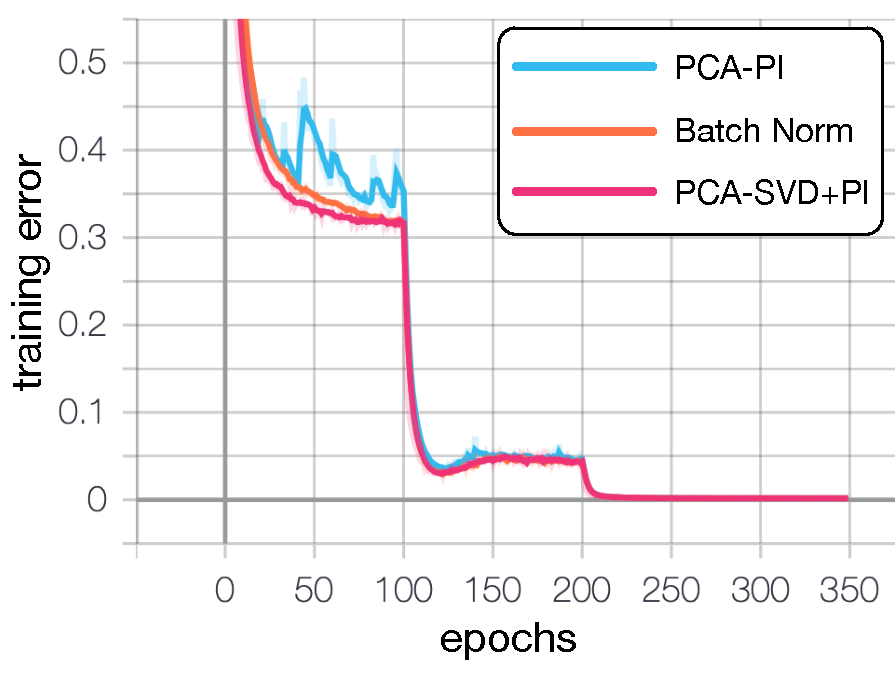
\includegraphics[width=\linewidth]{convergence.pdf}
}
{%
  \caption{Methods VS Performance.}%
}
\capbtabbox[\Xhsize]{%
\begin{tabular}{lcc}
\hline
Methods     & Min Error & Mean Error (5) \\ \hline
BN          & 4.66      & $4.81{\pm}0.19$   \\ \hline
PCA(PI)     & 5.05      & $5.35{\pm}0.25$ \\ \hline
PCA(SVD)    & NaN       & NaN                   \\ \hline
PCA(SVD+PI) & 4.58      & $\mathbf{4.67{\pm}0.06}$ \\ \hline
\\
\\
\\
\end{tabular}
}{%
  \caption{Methods VS Performance.}%
}
\end{floatrow}
\end{figure}


\begin{table}[!htb]
\begin{centering}
\begin{tabular}{|l|c|c|c|c|c|}
\hline
Norm Methods          & BN        & PCA(1 layer)   & ZCA(1 layer)  & PCA(1 block)   & ZCA(1 block) \\ \hline
Minimum Error         & 4.66      &  4.58  &   4.91 &  5.14 &  5.38\\ \hline
Mean Error (4) & $4.81{\pm}0.19$  &  $4.67{\pm}0.06$  & $5.02{\pm}0.28$ & $5.30{\pm}0.12$ & $5.50{\pm}0.10$ \\ \hline
\end{tabular}
\caption{CIFAR-10 test errors using ResNet18 (single PCA/ZCA normalization layer).}
\end{centering}
\end{table}
% !TEX root = ../top.tex
% !TEX spellcheck = en-US

\section{Conclusion}
\label{sec:conclusion}

% \subsubsection*{Acknowledgments}
% !TEX root = ../top.tex
% !TEX spellcheck = en-US

\section{Appendix}
\label{sec:appendix}
\section{Approximate SVD gradient with Power Iteration in backpropogation}
In the following 2 subsections, we will prove that when the gradient computed from Power Iteration equals to the gradients computed from SVD.
	\subsection{Gradient of Power Iteration}
	\label{sec: pi}
	To compute the leading eigenvector $\bv$ of $\bM$, Power Iteration uses the following standard formula,
	\begin{equation}
	\bv^{(k)} = \frac{\bM\bv^{(k-1)}}{\| \bM\bv^{(k-1)} \|},
	\end{equation}
	in which $\| {\cdot} \|$ denotes the $l_2$ norm, and $v^{(0)}$ is usually initialized randomly with  $\|v^{(0)}\|{=}1$.
    Its gradient formula is as follows~\cite{ye2017dynamic},
	\begin{equation}
	\begin{aligned} 
	\frac{\partial L}{\partial \bM} &=\sum_{k} \frac{\left(\bI-\bv^{(k+1)} \bv^{(k+1)\top}\right)}{\left\|\bM \bv^{(k)}\right\|} \frac{\partial L}{\partial \bv^{(k+1)}} \bv^{(k)\top} \\
	\frac{\partial L}{\partial \bv^{(k)}} &=\bM \frac{\left(\bI-\bv^{(k+1)} \bv^{(k+1)\top}\right)}{\left\|\bM \bv^{(k)}\right\|} \frac{\partial L}{\partial \bv^{(k+1)}} 
	\end{aligned}
	\end{equation}
	Using 3 power iteration steps for demonstration.
	\begin{equation}
	\begin{aligned} 
	\frac{\partial L}{\partial \bv^{(2)}} &=\bM \frac{\left(\bI-\bv^{(3)} \bv^{(3)\top}\right)}{\left\|\bM \bv^{(2)}\right\|} \frac{\partial L}{\partial \bv^{(3)}}\\
	\frac{\partial L}{\partial \bv^{(1)}} &=\bM \frac{\left(\bI-\bv^{(2)} \bv^{(2)\top}\right)}{\left\|\bM \bv^{(1)}\right\|} \frac{\partial L}{\partial \bv^{(2)}}
	=\bM \frac{\left(\bI-\bv^{(2)} \bv^{(2)\top}\right)}{\left\|\bM \bv^{(1)}\right\|} 
	\bM \frac{\left(\bI-\bv^{(3)} \bv^{(3)\top}\right)}{\left\|\bM \bv^{(2)}\right\|} \frac{\partial L}{\partial \bv^{(3)}}
	\end{aligned}
	\end{equation}
	
	Then the $\frac{\partial L}{\partial \bM}$ should be like the following, for the reason that we use eigenvalue decomposition (ED)'s result, denoted as $\bv$ as initial value, then $\bv {=} \bv^{(0)} {\approx}\bv^{(1)} {\approx} \bv^{(2)}{\approx} \cdots {\approx}\bv^{(k)}$. 
	
	\begin{equation}
	\begin{aligned} 
	\frac{\partial L}{\partial \bM}
	&{=}\frac{\left(\bI-\bv^{(3)} \bv^{(3)\top}\right)}{\left\|\bM \bv^{(2)}\right\|} \frac{\partial L}{\partial \bv^{(3)}} \bv^{(2)\top} +
	\frac{\left(\bI-\bv^{(2)} \bv^{(2)\top}\right)}{\left\|\bM \bv^{(1)}\right\|} \frac{\partial L}{\partial \bv^{(2)}} \bv^{(1)\top} + 
	\frac{\left(\bI-\bv^{(1)} \bv^{(1)\top}\right)}{\left\|\bM \bv^{(0)}\right\|} \frac{\partial L}{\partial \bv^{(1)}} \bv^{(0)\top}\\
	&{=} \left( \frac{\left(\bI {-} \bv \bv^{\top}\right)}{\left\|\bM \bv\right\|} {+}
	 \frac{\left(\bI {-} \bv \bv^{\top}\right) \bM  \left(\bI {-} \bv \bv^{\top}\right)}{\left\|\bM \bv\right\|^{2}}  {+} 
	 \frac{\left(\bI {-} \bv \bv^{\top}\right) \bM \left(\bI {-} \bv \bv^{\top}\right) \bM \left(\bI {-} \bv \bv^{\top}\right)}{\left\|\bM \bv\right\|^{3}} \right)
	 \frac{\partial L}{\partial \bv^{(3)}} \bv^{\top}
	\end{aligned}
	\label{eq: pi_expand}
	\end{equation}
	
	Known that $\bv \bv^{\top}$ and $\bM$ are symmetric and $\bM \bv = \lambda \bv$, we have 
$$\bv\bv^{\top}\bM = (\bM^{\top}\bv\bv^{\top})^{\top} = (\bM\bv\bv^{\top})^{\top} = (\lambda\bv\bv^{\top})^{\top} = \lambda\bv\bv^{\top} = \bM\bv\bv^{\top}.$$
	Introducing the equation above into the numerator in the second term of Eq.\ref{eq: pi_expand}, we can obtain:
	\begin{equation}
	\begin{aligned}
	\left(\bI - \bv \bv^{\top}\right) \bM  \left(\bI - \bv \bv^{\top}\right) &
	= \left(\bM - \bv \bv^{\top}\bM\right) \left(\bI - \bv \bv^{\top}\right) 
	=  \left(\bM - \bM \bv \bv^{\top}\right) \left(\bI - \bv \bv^{\top}\right) \\
	= \bM \left(\bI - \bv \bv^{\top}\right) \left(\bI - \bv \bv^{\top}\right) &
	= \bM \left(\bI - 2\bv \bv^{\top} + \bv \cancel{\left(\bv^{\top}\bv \right)} \bv^{\top}\right) 
	= \bM \left(\bI - \bv \bv^{\top} \right).
	\end{aligned}
	\label{eq: term1}
	\end{equation}
	Similarly, for the numerator in the third term in Eq.\ref{eq: pi_expand}, we have:
	\begin{equation}
	\left(\bI - \bv \bv^{\top}\right) \bM \left(\bI - \bv \bv^{\top}\right) \bM \left(\bI - \bv \bv^{\top}\right) = \bM \bM \left(\bI - \bv \bv^{\top} \right).
	\label{eq: term2}
	\end{equation}
	
Introducing Eq.\ref{eq: term1} and Eq.\ref{eq: term2} into Eq.\ref{eq: pi_expand}, we can obtain	
	\begin{equation}
	\frac{\partial L}{\partial \bM}
	 = \left( \frac{\left(\bI-\bv \bv^{\top}\right)}{\left\|\bM \bv\right\|} +
	 \frac{\bM \left(\bI-\bv \bv^{\top}\right)}{\left\|\bM \bv\right\|^{2}}  + 
	 \frac{\bM \bM \left(\bI-\bv \bv^{\top}\right)}{\left\|\bM \bv\right\|^{3}} \right)
	 \frac{\partial L}{\partial \bv^{(3)}} \bv^{\top}
	\label{eq: pi_3iter}
	\end{equation}

Extending the iteration number from 3 to $k$, Eq.\ref{eq: pi_expand} will be extended as
	\begin{equation}
	\frac{\partial L}{\partial \bM}
	 = \left( \frac{\left(\bI-\bv \bv^{\top}\right)}{\left\|\bM \bv\right\|}  +
	 \frac{\bM \left(\bI-\bv \bv^{\top}\right)}{\left\|\bM \bv\right\|^{2}}  + \cdots +
	 \frac{\bM^{k-1} \left(\bI-\bv \bv^{\top}\right)}{\left\|\bM \bv\right\|^{k}} \right) \frac{\partial L}{\partial \bv^{(k)}}
	\bv^{\top}
	\label{eq: pi_pytorch}
	\end{equation}	

Eq.\ref{eq: pi_pytorch} is the form we adopt to compute the gradients of SVD, and we set $k{=}19$.
	
	\subsection{Matrix Back-propagation}
	\label{sec: mbp}
	The analytic soltions of the gradients are from matrix back-propagation~\cite{ionescu2015matrix}.
	\begin{equation}
	\begin{aligned}
	\frac{\partial L}{\partial M}=V\left\{\left(\tilde{K}^{\top} \circ\left(V^{\top} \frac{\partial L}{\partial V}\right)\right)+\left(\frac{\partial L}{\partial \Sigma}\right)_{d i a g}\right\} V^{\top}
	\end{aligned}
	\end{equation}
	
	\begin{equation}
	\begin{aligned}
	\tilde{K}_{i j}=\left\{\begin{array}{ll}{\frac{1}{\lambda_{i}-\lambda_{j}},} & {i \neq j} \\ {0,} & {i=j}\end{array}\right.
	\end{aligned}
	\end{equation}
	
	\begin{equation}
	\begin{aligned}
	\tilde{K} = 
	\begin{bmatrix}
	0  &\frac{1}{\lambda_{1} - \lambda_{2}} &\frac{1}{\lambda_{1} - \lambda_{3}} &\cdots &\frac{1}{\lambda_{1} - \lambda_{n}}\\
	\frac{1}{\lambda_{2} - \lambda_{1}} &0 &\frac{1}{\lambda_{2} - \lambda_{3}} &\cdots &\frac{1}{\lambda_{2} - \lambda_{n}}\\
	\frac{1}{\lambda_{3} - \lambda_{1}} &\frac{1}{\lambda_{3} - \lambda_{2}} &0 &\cdots &\frac{1}{\lambda_{3} - \lambda_{n}}\\
	\vdots &\vdots &\vdots &\ddots &\vdots\\
	\frac{1}{\lambda_{n} - \lambda_{1}} &\frac{1}{\lambda_{n} - \lambda_{2}} &\frac{1}{\lambda_{n} - \lambda_{3}} &\cdots &0
	\end{bmatrix}
	\end{aligned}
	\end{equation}
	where $\lambda_{i}$ is the eigen-value.
	
	\begin{equation}
	\begin{aligned}
	V = 
	\begin{bmatrix}
	\bv_{1} &\bv_{2} &\bv_{3} &\cdots &\bv_{n}
	\end{bmatrix}
	\end{aligned}
	\end{equation}
	where $v_{i}$ is the eigen-vector.
	
	\begin{equation}
	\begin{aligned}
	\frac{\partial L}{\partial V} = 
	\begin{bmatrix}
	\frac{\partial L}{\partial \bv_{1}} &\frac{\partial L}{\partial \bv_{2}}  &\frac{\partial L}{\partial \bv_{3}}  &\cdots &\frac{\partial L}{\partial \bv_{n}} \\
	\end{bmatrix}
	\end{aligned}
	\end{equation}
	
	\begin{equation}
	\begin{aligned}
	V^{\top}\frac{\partial L}{\partial V} = 
	\begin{bmatrix}
	\bv_{1}^{\top}\frac{\partial L}{\partial \bv_{1}} &\bv_{1}^{\top}\frac{\partial L}{\partial \bv_{2}}  &\bv_{1}^{\top}\frac{\partial L}{\partial \bv_{3}}  &\cdots &\bv_{1}^{\top}\frac{\partial L}{\partial \bv_{n}} \\
	\bv_{2}^{\top}\frac{\partial L}{\partial \bv_{1}} &\bv_{2}^{\top}\frac{\partial L}{\partial \bv_{2}}  &\bv_{2}^{\top}\frac{\partial L}{\partial \bv_{3}}  &\cdots &\bv_{2}^{\top}\frac{\partial L}{\partial \bv_{n}} \\
	\bv_{3}^{\top}\frac{\partial L}{\partial \bv_{1}} &\bv_{3}^{\top}\frac{\partial L}{\partial \bv_{2}}  &\bv_{3}^{\top}\frac{\partial L}{\partial \bv_{3}}  &\cdots &\bv_{3}^{\top}\frac{\partial L}{\partial \bv_{n}} \\
	\vdots &\vdots &\vdots &\ddots &\vdots\\
	\bv_{n}^{\top}\frac{\partial L}{\partial \bv_{1}} &\bv_{n}^{\top}\frac{\partial L}{\partial \bv_{2}}  &\bv_{n}^{\top}\frac{\partial L}{\partial \bv_{3}}  &\cdots &\bv_{n}^{\top}\frac{\partial L}{\partial \bv_{n}} \\
	\end{bmatrix}
	\end{aligned}
	\end{equation}
	
	\begin{equation}
	\begin{aligned}
	\tilde{K}\circ V^{\top}\frac{\partial L}{\partial V} = 
	\begin{bmatrix}
	0& \frac{1}{\lambda_{2} - \lambda_{1}}\bv_{1}^{\top}\frac{\partial L}{\partial \bv_{2}}  
	&\frac{1}{\lambda_{3} - \lambda_{1}}\bv_{1}^{\top}\frac{\partial L}{\partial \bv_{3}}  
	&\cdots &\frac{1}{\lambda_{n} - \lambda_{1}}\bv_{1}^{\top}\frac{\partial L}{\partial \bv_{n}} \\
	\frac{1}{\lambda_{1} - \lambda_{2}}\bv_{2}^{\top}\frac{\partial L}{\partial \bv_{1}} &0  
	&\frac{1}{\lambda_{3} - \lambda_{2}}\bv_{2}^{\top}\frac{\partial L}{\partial \bv_{3}}  &\cdots 
	&\frac{1}{\lambda_{n} - \lambda_{2}}\bv_{2}^{\top}\frac{\partial L}{\partial \bv_{n}} \\
	\frac{1}{\lambda_{1} - \lambda_{3}}\bv_{3}^{\top}\frac{\partial L}{\partial \bv_{1}} 
	&\frac{1}{\lambda_{2} - \lambda_{3}}\bv_{3}^{\top}\frac{\partial L}{\partial \bv_{2}}  &0  &\cdots 
	&\frac{1}{\lambda_{n} - \lambda_{3}}\bv_{3}^{\top}\frac{\partial L}{\partial \bv_{n}} \\
	\vdots &\vdots &\vdots &\ddots &\vdots\\
	\frac{1}{\lambda_{1} - \lambda_{n}}\bv_{n}^{\top}\frac{\partial L}{\partial \bv_{1}} 
	&\frac{1}{\lambda_{2} - \lambda_{n}}\bv_{n}^{\top}\frac{\partial L}{\partial \bv_{2}} 
	 &\frac{1}{\lambda_{3} - \lambda_{n}}\bv_{n}^{\top}\frac{\partial L}{\partial \bv_{3}}  &\cdots &0 \\
	\end{bmatrix}
	\end{aligned}
	\end{equation}
	
	\begin{equation}
	\begin{aligned}
	V \tilde{K}\circ V^{\top}\frac{\partial L}{\partial V} &=
	\begin{bmatrix}
	\sum_{i\neq 1}^{n}\frac{1}{\lambda_{1}-\lambda_{i}}\bv_{i}\bv_{i}^{\top}\frac{\partial L}{\partial \bv_{1}},
	& \sum_{i\neq 2}^{n}\frac{1}{\lambda_{2}-\lambda_{i}}\bv_{i}\bv_{i}^{\top}\frac{\partial L}{\partial \bv_{2}}, 
	&\cdots,
	&\sum_{i\neq n}^{n}\frac{1}{\lambda_{n}-\lambda_{i}}\bv_{i}\bv_{i}^{\top}\frac{\partial L}{\partial \bv_{n}}
	\end{bmatrix}
	\end{aligned}
	\end{equation}	
	
	\begin{equation}
	V \tilde{K}\circ V^{\top}\frac{\partial L}{\partial V} V^{\top} =
	\sum_{i\neq 1}^{n}\frac{1}{\lambda_{1}-\lambda_{i}}\bv_{i}\bv_{i}^{\top}\frac{\partial L}{\partial \bv_{1}} \bv_{1}
	+ \sum_{i\neq 2}^{n}\frac{1}{\lambda_{2}-\lambda_{i}}\bv_{i}\bv_{i}^{\top}\frac{\partial L}{\partial \bv_{2}} \bv_{2}
	+\cdots
	+\sum_{i\neq n}^{n}\frac{1}{\lambda_{n}-\lambda_{i}}\bv_{i}\bv_{i}^{\top}\frac{\partial L}{\partial \bv_{n}} \bv_{n}
	\end{equation}	
	
	\begin{equation}
    V\left(\frac{\partial L}{\partial \Sigma}\right)_{d i a g} V^{\top} = \sum_{i=1}^n \frac{\partial L}{\partial \lambda_i}\bv_{i}\bv_{i}^{\top}
	\end{equation}    	
	
	%We do not use eigenvalues in the forward pass, so that it has no gradients, which means $\frac{\partial L}{\partial \Sigma}=0$.
	Now let's consider the partial derivative \emph{w.r.t} dominant eigenvector $\bv_{i}$ and ignore the rest $\frac{\partial L}{\partial \bv_{i}}, i \neq 1$.
	Then $\frac{\partial L}{\partial M}$ would be,
	
	\begin{equation}
	\frac{\partial L}{\partial M}=\sum_{i=2}^{n}\frac{1}{\lambda_{1}-\lambda_{i}}\bv_{i}\bv_{i}^{\top}\frac{\partial L}{\partial \bv_{1}}\bv_{1}^{\top} + \frac{\partial L}{\partial \lambda_1}\bv_{1}\bv_{1}^{\top}
	\end{equation}
If the network does not involve the eigenvalues, the derivative of the eigenvalues will be 0 and it could be ignored. In other words, the second term in the equation above could be ignored.
Now we have shown that the partial derivative of \emph{e.g.}, $\bv_1$ computed from Power Iteration and SVD share the same form when $k\rightarrow \inf$.
Similar deductions could be done for  $\bv_i, i=2,3,\cdots, n$.




\small

\medskip
\small
\bibliographystyle{unsrt}
\bibliography{neurips_2019.bib}

\end{document}
